\documentclass[]{article}
\usepackage{lmodern}
\usepackage{amssymb,amsmath}
\usepackage{ifxetex,ifluatex}
\usepackage{fixltx2e} % provides \textsubscript
\ifnum 0\ifxetex 1\fi\ifluatex 1\fi=0 % if pdftex
  \usepackage[T1]{fontenc}
  \usepackage[utf8]{inputenc}
\else % if luatex or xelatex
  \ifxetex
    \usepackage{mathspec}
  \else
    \usepackage{fontspec}
  \fi
  \defaultfontfeatures{Ligatures=TeX,Scale=MatchLowercase}
\fi
% use upquote if available, for straight quotes in verbatim environments
\IfFileExists{upquote.sty}{\usepackage{upquote}}{}
% use microtype if available
\IfFileExists{microtype.sty}{%
\usepackage[]{microtype}
\UseMicrotypeSet[protrusion]{basicmath} % disable protrusion for tt fonts
}{}
\PassOptionsToPackage{hyphens}{url} % url is loaded by hyperref
\usepackage[unicode=true]{hyperref}
\hypersetup{
            pdftitle={Fertility Issues in Developing Countries},
            pdfauthor={Claus C Pörtner Department of Economics Albers School of Business and Economics Seattle University, P.O. Box 222000 Seattle, WA 98122 cportner@seattleu.edu www.clausportner.com \& Center for Studies in Demography and Ecology University of Washington},
            pdfborder={0 0 0},
            breaklinks=true}
\urlstyle{same}  % don't use monospace font for urls
\usepackage{graphicx,grffile}
\makeatletter
\def\maxwidth{\ifdim\Gin@nat@width>\linewidth\linewidth\else\Gin@nat@width\fi}
\def\maxheight{\ifdim\Gin@nat@height>\textheight\textheight\else\Gin@nat@height\fi}
\makeatother
% Scale images if necessary, so that they will not overflow the page
% margins by default, and it is still possible to overwrite the defaults
% using explicit options in \includegraphics[width, height, ...]{}
\setkeys{Gin}{width=\maxwidth,height=\maxheight,keepaspectratio}
\IfFileExists{parskip.sty}{%
\usepackage{parskip}
}{% else
\setlength{\parindent}{0pt}
\setlength{\parskip}{6pt plus 2pt minus 1pt}
}
\setlength{\emergencystretch}{3em}  % prevent overfull lines
\providecommand{\tightlist}{%
  \setlength{\itemsep}{0pt}\setlength{\parskip}{0pt}}
\setcounter{secnumdepth}{0}
% Redefines (sub)paragraphs to behave more like sections
\ifx\paragraph\undefined\else
\let\oldparagraph\paragraph
\renewcommand{\paragraph}[1]{\oldparagraph{#1}\mbox{}}
\fi
\ifx\subparagraph\undefined\else
\let\oldsubparagraph\subparagraph
\renewcommand{\subparagraph}[1]{\oldsubparagraph{#1}\mbox{}}
\fi

% set default figure placement to htbp
\makeatletter
\def\fps@figure{htbp}
\makeatother


\title{Fertility Issues in Developing Countries}
\author{Claus C Pörtner\\
Department of Economics\\
Albers School of Business and Economics\\
Seattle University, P.O. Box 222000\\
Seattle, WA 98122\\
\href{mailto:cportner@seattleu.edu}{\texttt{cportner@seattleu.edu}}\\
\href{http://www.clausportner.com}{\texttt{www.clausportner.com}}\\
\&\\
Center for Studies in Demography and Ecology\\
University of Washington\\}
\date{April 2017}

\begin{document}
\maketitle

\section{Introduction}\label{introduction}

Despite a common perception that fertility is very high in developing countries, the truth is substantially more complicated. Figure {[}fig:TFR{]} shows that there has been an astonishing decline in most developing countries' total fertility rate (TFR) over the last half century.\footnote{TFR is the number of children a women entering her reproductive life would have if she had children following the age-specific fertility rates observed at that point in time. Hence, it is composite or snapshot measure of current fertility behavior.} Half a decade ago, TFR was around 7 children, with the exception of Europe and Central Asia. The most recent data show, however, that, with the exception of Sub-Saharan African, TFR is now either below or only slightly above the replacement level of 2.1. Despite this rapid decline in fertility population size is still growing in many of these regions because there are still many more young people than older people and these young people either have not entered reproductive age or are just starting out.

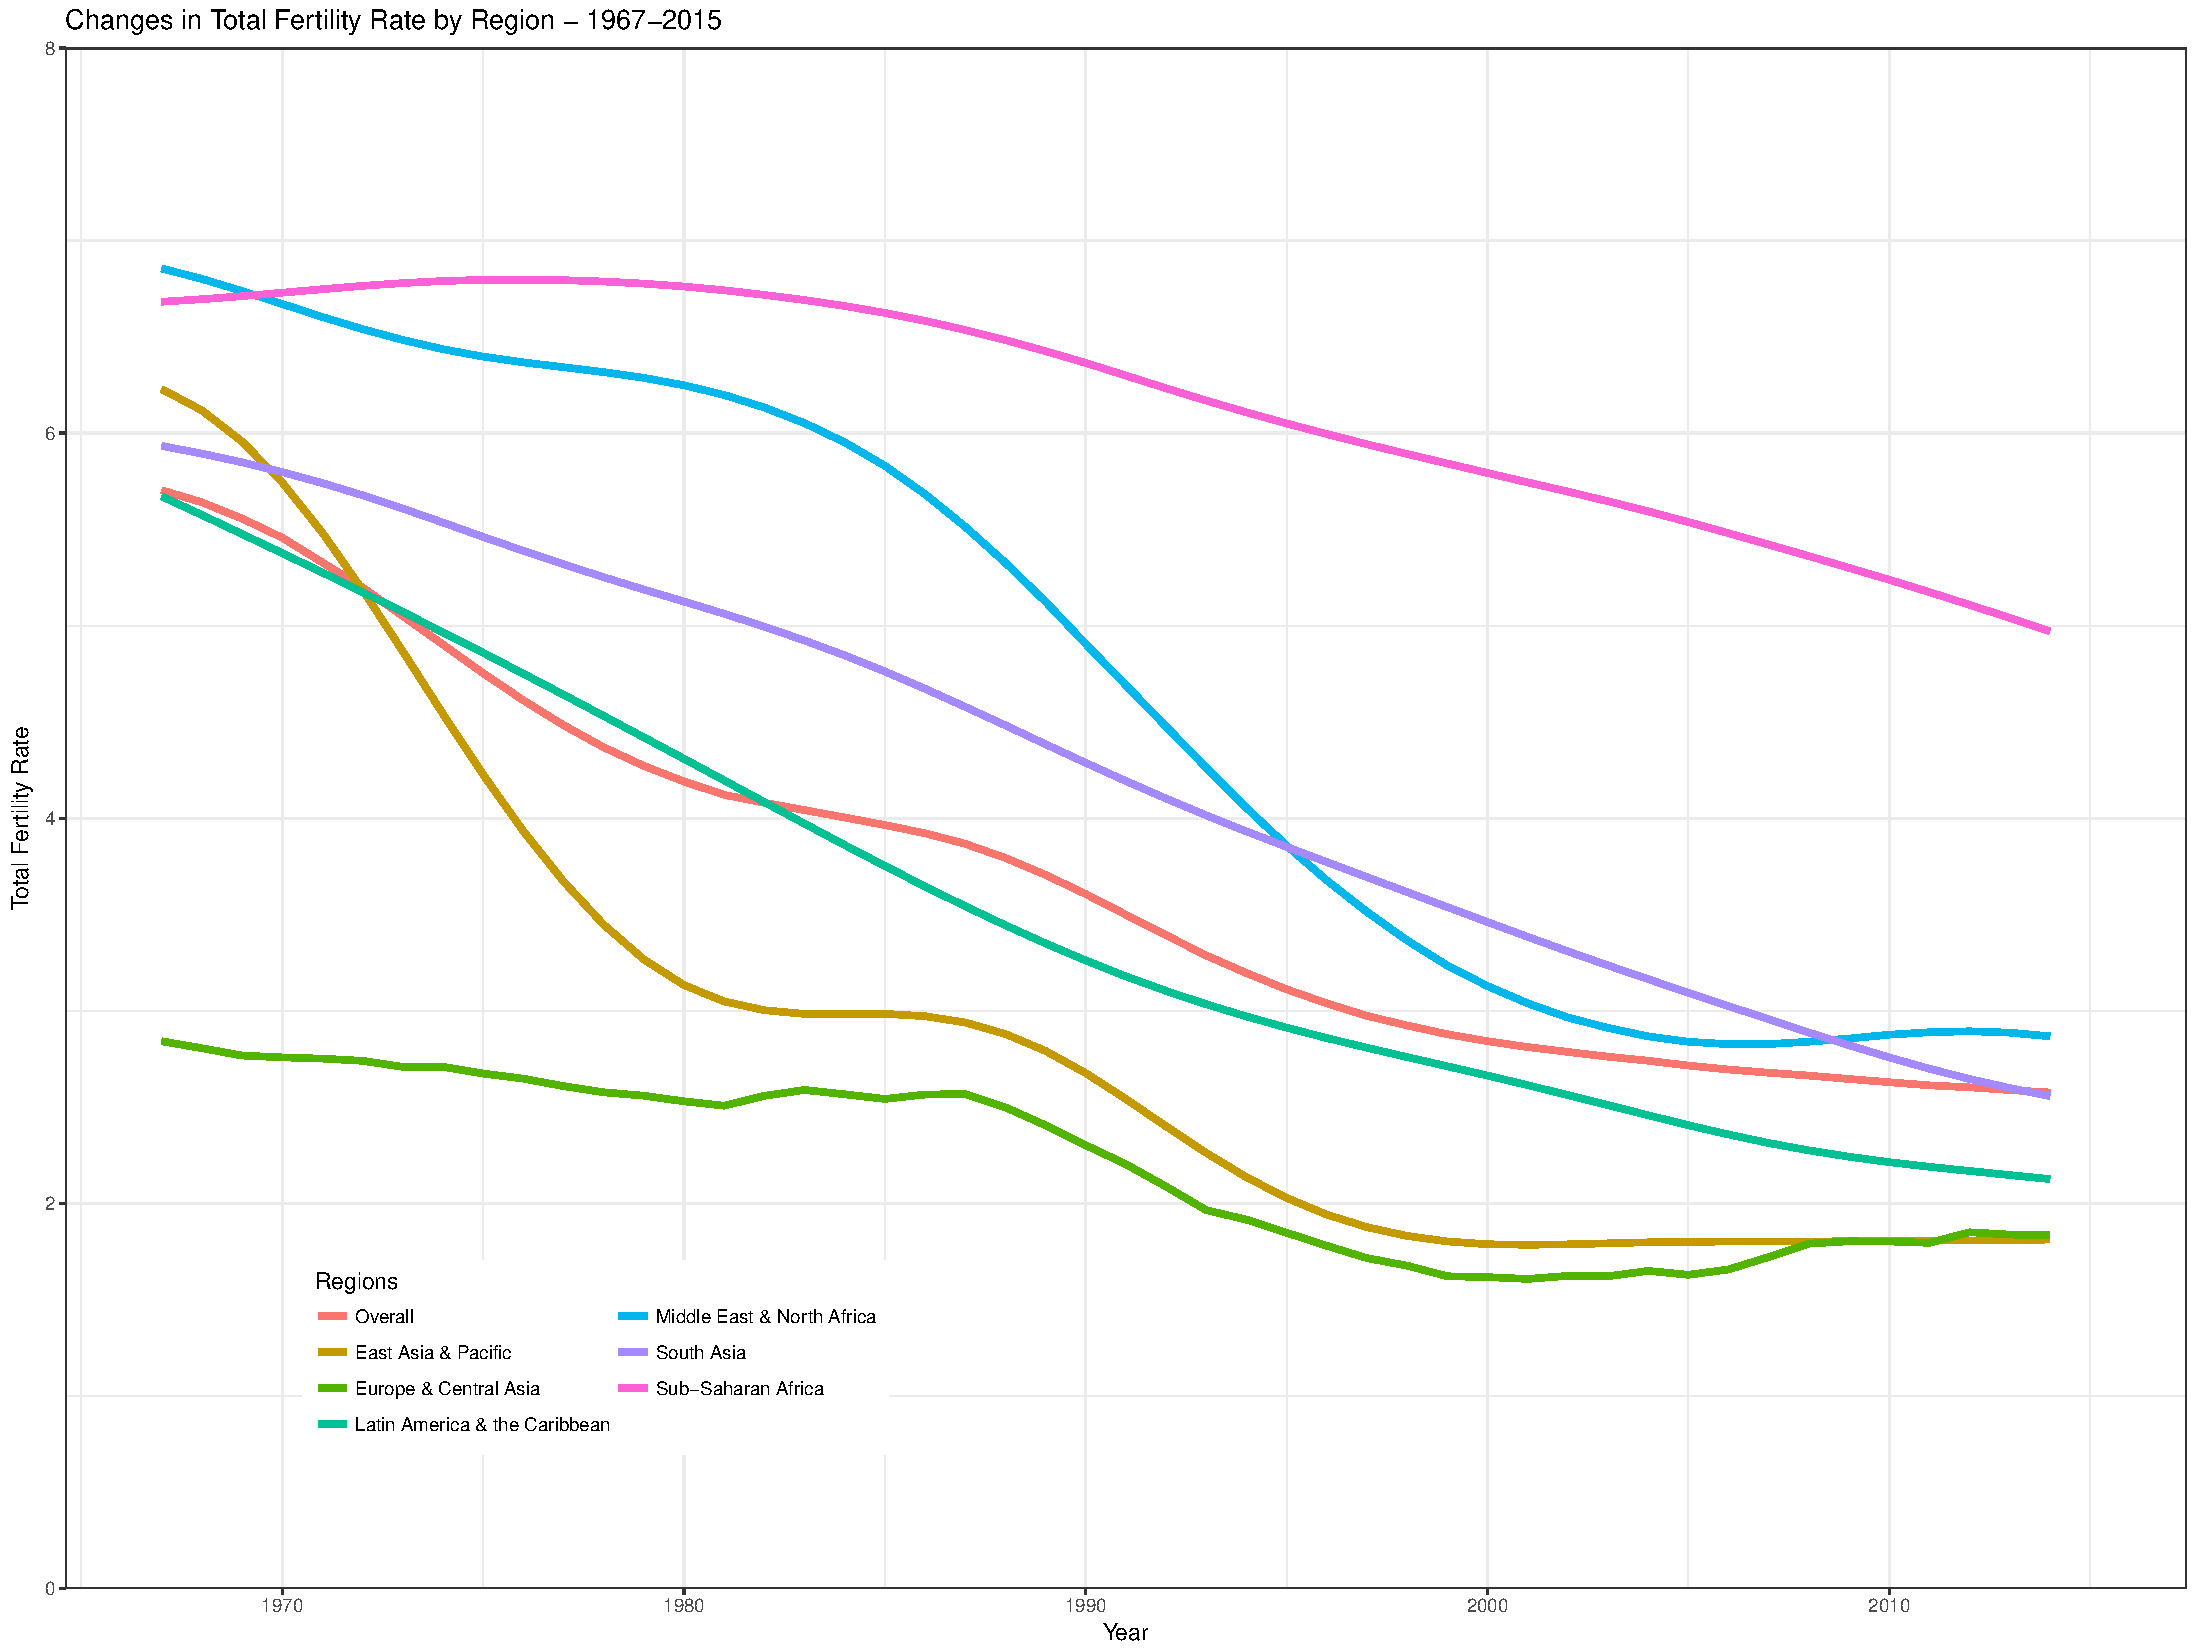
\includegraphics{../figures/totalFertilityRates.pdf} {[}fig:TFR{]}

If fertility levels are close to identical across developing and developed countries and there is rapid urbanization and increasing labor force participation among women do we even need a developing country version of this chapter? The goal of this chapter is to highlight areas in which a separate focus on developing countries is still relevant, what the recent developments in research has been, and most importantly, what I consider to be the main outstanding issues.

\section{Sub-Saharan Africa}\label{sub-saharan-africa}

The outlier in the figure above is Sub-Saharan Africa. Sub-Saharan Africa now has an average TFR that is about twice as large as the other regions. Most of the projected future increase in world population is therefore likely to come from Sub-Saharan Africa (Gerland et al. 2014).\footnote{Currently Africa is home to about 1 billion people, but this will increase to between 3.1 and 5.7 billion by the end of the century.} The most important issues from a policy standpoint is why the fertility decline in Sub-Saharan Africa have moved at a much slower pace than the other regions and even appears to have stalled in some countries (Ainsworth 1996; Singh, Bankole, and Darroch Forthcoming). The purpose of this section is not to provide the final answer, but instead to highlight both how we can think about fertility decisions and suggest possible answers.

Broadly speaking there are two competing approaches to explaining fertility decisions.\footnote{This is clearly a simplification but it serves to illustrate the differences in approaches.} One sees fertility preferences as the main driver of fertility and considers preferences malleable and mainly determined by cultural factors and transmission of ideas of ideal family size across groups. Under this approach the main constraints on reaching desired fertility is the level of access to family planning and contraceptives.

The other sees the decision on fertility as driven by the trade-off between the cost of children and the return to children, which can either be monetary or the utility of having offspring. In this approach parents are assumed to be able to control fertility even in the absence of modern contraceptives. Hence, although lower cost of preventing births---for example easier access to modern contreceptive---will still lower fertility in this approach the decline in fertility is assumed to be much smaller than the first theory.

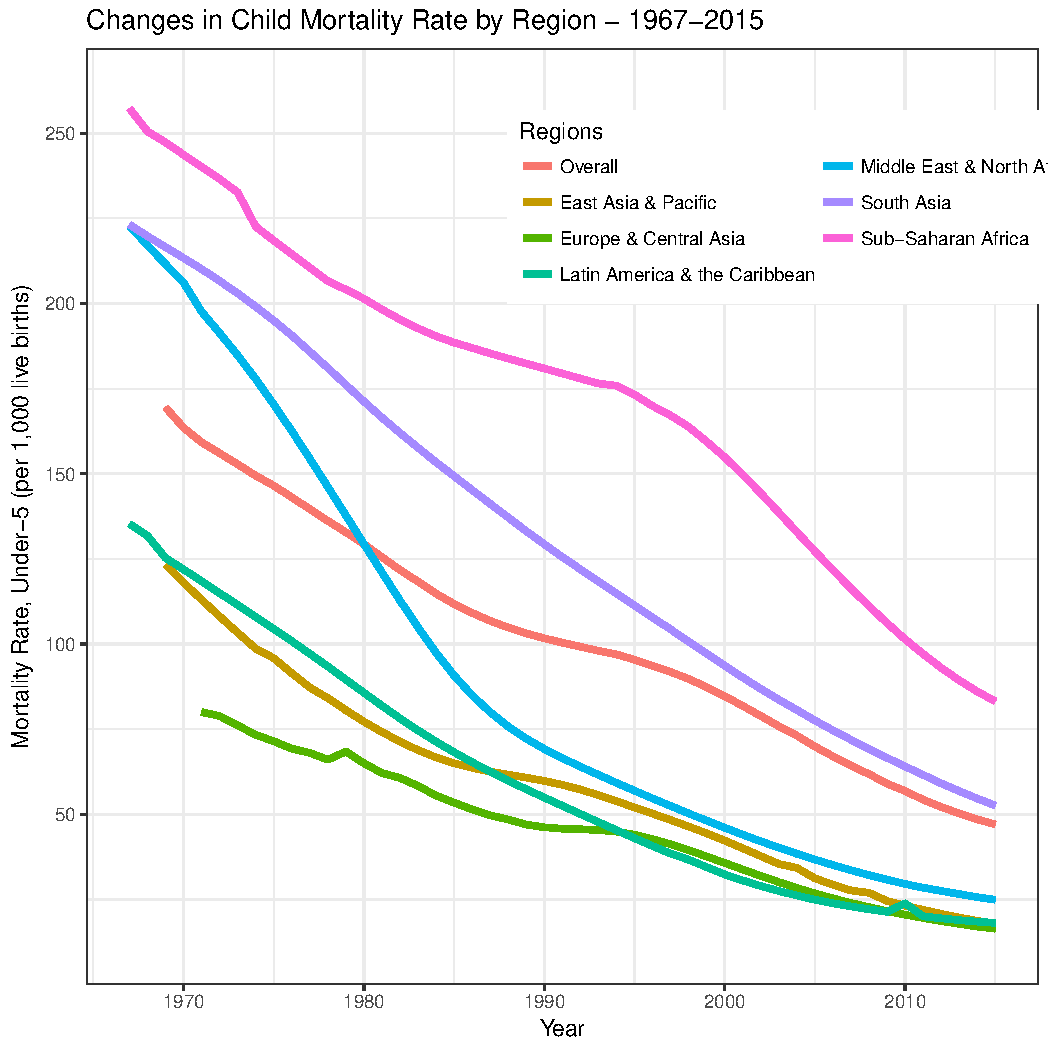
\includegraphics{../figures/childMortalityRates.pdf} {[}fig:mortality{]}

Both theories consider the surviving number of children as the main outcome that people are interested in. One possible explanation for the slow decline in fertility could therefore be that mortality in Sub-Saharan Africa is higher than in the other regions. Figure {[}fig:mortality{]} shows the development over time in under-5 mortality across the same regions as above. The improvements in mortality risk over time are truly astonishing. Over the last half-decade under-5 mortality in developing countries has fallen from close to 175 to below 50 per 1,000 live births. Sub-Saharan Africa, however, lacks substantially behind other regions. Despite a massive improvement from a situation where more than a quarter of all children born did not live to see their fifth birthday to about 80 deaths per 1,000 births, the current mortality rate is still more than three times larger than that of the other regions (with the exception of Middle East and North Africa). Although mortality is likely part of the explanation it cannot be the full explanation. Mortality in Sub-Saharan Africa is at the same level as it was in South Asia around the turn of the century, but fertility is about 1.5 child higher in Sub-Saharan Africa than it was in South Asia at the turn of the century (and therefore at the same level of mortality).

If mortality is not the explanation, what might lead to the higher fertility in Sub-Saharan Africa? Demographers, following the first approach described above, have argued that the two main reasons for the slow decline in fertility in Sub-Saharan Africa are the high ideal family size still in place and a substantial ``unmet need'' for contraception (Bongaarts and Casterline 2013; Singh, Bankole, and Darroch Forthcoming). Contraceptive use is, indeed, lower in Sub-Saharan Africa than the other regions, but other regions managed to reduced fertility even in the absence of access to modern contraceptives Schultz (1985; Galloway 1987; Bailey and Chambers 1998; Bengtsson and Dribe 2006). Furthermore, one difference in fertility behavior between Sub-Saharan Africa and the other regions are that the longer birth intervals even in the absence of access to modern contraception, which are the result of postpartum sexual abstinence and extended periods of breastfeeding (Caldwell, Orubuloye, and Caldwell 1992). To the extend that the longer birth intervals are the result of conscious decisions it shows that people are able to control fertility.\footnote{It is still possible that fertility is higher than desired because the higher cost of preventing ``accidental'' conceptions. This would explain why the estimated effect of access to family planning in Ethiopia shows a reduction in fertility of about one birth, which is equivalent to an approximate 20\% reduction in fertility Pörtner, Beegle, and Christiaensen (2014).}

There are three alternative explanation that may explain the slow decline. First, the relative abundance of land compared to other regions. Second, low levels of education; or at least low levels of quality in education. Finally, the role of urbanization across regions.

The effect of land access on fertility works in a couple of different way. First, there is more land per capita in Sub-Saharan Africa than in the other regions. At the median projected population growth for Sub-Saharan Africa---which is 4.2 billion people by 2100---the population density will only be roughly equal to that of China today (Gerland et al. 2014 p 235). The low density means that there is little pressure to restrain fertility for fear of running out of land. In fact, it is likely that there is a higher return to children in Sub-Saharan Africa than in the other regions---or, at least, a substantially lower cost---because the return to children working on the family farm is higher (Caldwell, Orubuloye, and Caldwell 1992). Similarly, there are substantially higher return to having wives work on agricultural land (Jacoby 1995). The associated polygyny also appeared to have resulted in a situation where the cost of the children where born by the individual wives, but the decision on fertility was made by the husband. I return to this point below.

A second characteristics of land in Sub-Saharan Africa that also can lead to higher fertility is that---despite its abundance---access to land rights are controlled at the local level by chiefs and other local institutions rather than through market based buying and selling of land. This is important because the main way to maintain land fertility in many places in Sub-Saharan Africa is through fallowing and with less secure land rights farmers may fallow their land for shorter periods than those with more secure rights (Goldstein and Udry 2008).\footnote{See also Besley (1995), who discuss other investments in land that can secure property rights.} The reason unsecure land rights can lead to other fertility is that land is often allocated based on the number of household members. Hence, more children, everything else equal, will increase your claim on land access. The irony here is, of course, that if everybody else follows the same strategy the result will be much higher fertility and little change in the allocation of land. For both of these potential effects of land access on fertility we, however, have little direct information on their effects and a this is one area that calls out for future research.

My second suggestion for a major factor impacting fertility in Sub-Saharan Africa is education. The standard economic model of fertility considers the opportunity cost of women's time to be the main factor affecting the number of children (Becker 1991). As women gain more education the cost of their time, and therefore of childbearing and childrearing, increases reducing fertility and leads to better health outcomes for both women and children.\footnote{It is, however, not completely clear why there is such a strong association between education and health (Thomas, Strauss, and Henriques 1991; Glewwe 1999; Kovsted, Pörtner, and Tarp 2002)} The better health outcomes lead to lower child mortality, which in turn further decreases fertility because fewer births are required to reach a desired number of surviving children (Ainsworth, Beegle, and Nyamete 1996). The effect of education on fertility is essentially universal, making it the main recommended way to decrease fertility (Schultz 2002).

Fertility, however, begins to decline at higher levels of education in Sub-Saharan Africa than in other regions and the relationship between fertility and education may even be positive for low levels of education (Ainsworth, Beegle, and Nyamete 1996; Benefo and Schultz 1996; Thomas and Maluccio 1996). Part of the problem may be the quality of education in Sub-Saharan Africa. In other words, the stated number of years of education may be worse predictor of actual human capital accumulation in Sub-Saharan Africa than other regions.

A good example of this problem is Tanzania (Galabawa 2001; Wedgwood 2005). Taken at face value, Tanzania has a very high reported education level. This is most likely the result of the 1974 Universal Primary Education Movement, which increased accessibility of primary education and enrollment rates. The problem is that the quality of education reportedly was very low. In addition, the crisis Tanzania experienced in the 1980s further lowered the quality and enrollments declined significantly. Hence, it is unclear to what extent reported education levels reflect women's actual human capital. The result is that education does not appear to have as a substantial effect on fertility in Tanzania as other found elsewhere Alam and Pörtner (2016).

The final explanation for differences in TFRs across regions is the role of urbanization. When talking about fertility and its determinants in Sub-Saharan Africa one discussion seems to be essentially absent and that is the difference between urban and rural areas. As a rule all regions have had and have higer fertility in rural areas than in urban areas. This is directly in line with what we expect. The cost of children is clearly higher in urban areas than in rural areas, even for women with the same amount of education---and therefore the same opportunity cost of time. Sub-Saharan Africa is no difference. An example is Ethiopia in 2011, where the overall TRF is 4.8, but that covers a TFR of 5.5 in rural areas and only 2.6 in urban areas (Central Statistical Agency/Ethiopia and ICF International 2012). Part of the explanation for the lower fertility is the higher average education level of women in urban areas than in rural areas. But, even for women with the same education level fertility is lower in urban areas than in rural areas (Ainsworth, Beegle, and Nyamete 1996).

There has, however, not been a systematic examination of how fertility varies with education in urban areas across different regions. If predicted fertility is similar across regions for the same level of education that would suggest that Sub-Saharan Africa is not inherently different. A lower ``return'' to education could either be an indication that the quality of education is lower, that the opportunity cost increases with higher education is not as high in Sub-Saharan Africa as in other areas (either because of the lower quality or because of lower levels of development), or it could suggest that there is something inherently different in what determines fertility in Sub-Saharan Africa than in other regions.

\section{Timing of Fertility}\label{timing-of-fertility}

How couple time their births is relevant both because it provides us with an idea of how good people are at controlling their fertility and because timing of births may impact the health of both mother and children. We know, however, surprisingly little about what determines the timing of births in developing countries. Especially with more and more women entering the labor force in developing countries, understanding how timing decisions are made will be important for the design of suitable policies. The lack of research is partly because of data limitations and partly because of the difficulty in identifying the causal relationship between timing and other decisions, such as labor supply.

The three sub-areas where we do have some information is the timing of first birth, how births respond to shocks, and how the sex of the last child affect timing of the next birth. This section covers the timing of first birth and leaves the two other areas for the sections below.

Having your first birth earlier in life is generally associated with lower educational attainment, higher completed fertility, and worse health and labor outcomes. This is, however, not necessarily indicative of a causal relationship between earlier first birth and the other outcomes. A woman who, for example, has a lower expected return to education may decide that using contraceptive is not worth the cost and therefore would be more likely to conceive and subsequently drop out of school. Furthermore, as long as fertility is well below natural fertility levels having an earlier birth will not, in itself, increase your fertility.\footnote{Natural fertility is the level of fertility that would prevail in a population that makes no conscious effort to limit, regulate, or control fertility.}

For this reason most of the literature has focused mainly on what determines the timing of first births---and to some extent on whether women are more likely to drop out of school after their first birth. In the relatively small literature on timing of first births there are two main approaches to trying to identify whether a causal relationship exists between timing of first birth and other outcomes. One is to look for variables that can be argued to only affect one of the other, with no direct effect on the other outcomes, and jointly estimate the various decisions.\footnote{This approach is often combined with restrictions on the correlation of error terms across decisions} The other approach is experimental where researchers randomly access to a program that is believe to influence one of decisions and then examine whether the timing of births and the other outcomes are affected by the program. The downside of both approaches is that we cannot learn much about what completed fertility is going to look like. Even experiments that follow people for an extended period, like the seven years in Duflo, Dupas, and Kremer (2015), only gets to the beginning of the prime childbearing years, 20 to 30. Independent of method, the results suggest that increasing education is important in delaying marriage and first birth (Duflo, Dupas, and Kremer 2015; Marchetta and Sahn 2016) An important caveat is, however, the effects of interventions may disappear quickly after the end of the program (Baird, McIntosh, and Özler 2016).

\section{Bargaining Power and Sex Preference}\label{bargaining-power-and-sex-preference}

An important question is what happens when husband and wife do not agree on the desired number of children they have. The originally literature on this question mainly showed that families do not necessarily behave as if husband and wife have similar preference. One way to get at this is to look at unearned income that can attributed to either the wife and husband. If the number of children born changes with shifts in the distribution of unearned income that indicates that the partners have different preferences.

Results from Thailand show that women with more ``bargaining power'' spent less time working and preferred to have more children (Schultz 1990). The result that women prefer more children is not generally supported and in most cases men have a higher preferred number of children than women (Westoff 2010). An example of this is Malaysia where both ethnic Chinese and ethnic Malay husbands had a higher ideal number of children than their wives; although the ideal numbers where below the actual number of children for both partners(Rasul 2008).

Sub-Saharan Africa is often considered a special case when it comes to different preferences for ideal number of children across husband and wife. The father bears less of the cost of children than in other places because of the family structure, especially in West Africa (Caldwell, Orubuloye, and Caldwell 1992). It would seem that in cases like this, it would be beneficial to provide women with more control over use of contraceptives. An experiment in Zambia tried exactly that (Ashraf, Field, and Lee 2014). One group of women where given an individual voucher for free and immediate access contraceptives and, because the most popular contraceptives is injectables, the ability to hide contraceptive use from their partners if they wanted to. In the other group the husband were handed the vouchers and both the husband's and wife's signatures were required to redeem it. As expected, the women who needed their husband's signature were less likely to visit a family planning nurse and less likely to use injectable contraceptives. As a result these women were also more likely to have a birth. The caveat is that women who could potential conceal their use of contraceptives reported significant reductions in happiness, health, and ease of mind compared to the women in the group where both signatures were required.

When discussing difference in preferred number of children across men and women it is important to realize the is evidence that men, in fact, end up with more children (Field et al. 2016). Using data from eight Sub-Saharan African countries, men have, on average, more children than women of the same cohort in seven out of the eight countries. The gaps are large, ranging from 0.8 children in Zambia to 4.6 children in Burkina Faso, but appear to be decreasing over time. This pattern is consistent with men partnering with younger women in a situation where the population is growing and with polygyny. This means that that differences in desired number of children are often mirrored in differences in actual achieved fertility. The implication is that there might not be an innate contradiction surrounding fertility behavior within couples (Field et al. 2016).

\subsection{Sex Preference}\label{sex-preference}

An especially important aspect of intrahousehold allocation is the preference for children of a specific sex. The dominant version is a strong preference for sons in many countries; most notably in India and China. The literature is somewhat fuzzy on what exactly constitutes son preference. One popular version is that for their ideal number of children, parents would prefer to have more sons than daughters, and the strength of son preference is then measured by how many more sons than daughters a family wants. This measure of son preference is commonly used in the literature (Clark 2000; Jensen and Oster 2009; Hu and Schlosser 2015 See, for example,). Other versions are possible. Parents might, for example, have a preference for one son, but once that one son is secured they do not have strong preferences for the distribution between sons and daughters for the remaining children.

Before prenatal sex determination became available, most research focused on the impact of son preference on fertility decision and spacing between births. This literature showed clearly that in areas with son preference families were more likely to stop childbearing after the birth of a son than after the birth of a daughter (see, for example, Das 1987; Arnold 1997; Clark 2000).\footnote{Filmer, Friedman, and Schady (2009) analyse the relationship between the sex composition of previous children and subsequent fertility behavior using data from 64 countries.} Furthermore, in the absence of sex-selective abortions, son preference often leads to a shorter duration until the next birth if the previous birth was a daughter (see, for example, Das 1987; Rahman and DaVanzo 1993; Pong 1994; Haughton and Haughton 1996; Arnold 1997). The resulting shorter spacing is thought to be associated with worse health outcomes for the girls (Arnold, Choe, and Roy 1998; Whitworth and Stephenson 2002; Rutstein 2005; Conde-Agudelo, Rosas-Bermúdez, and Kafury-Goeta 2006). There is also evidence that girls were underreported in China as a result of strong son preference combined with the one-child policy (Merli and Raftery 2000).

With the introduction of amniocentesis, ultrasound, and CVS it became possible to tell the sex of a fetus and abort the pregnancy if the fetus did not have the preferred sex. By itself, this may not have led to substantial changes, but combined with lower desired fertility as in India or forced lower fertility as in China the availability of prenatal sex determination had substantial impacts on the sex ratio. It is easy to see how declining fertility can increase the use of sex selection. Take a family that wants one son. If the family is willing to have up to 4 children, the probability of having a son is more than 94 percent, even without sex selection, and that increases to almost 99 percent if the family is willing to have up to 6 children.\footnote{The probabilities of not having a son are 48.8 percent for one child, 23.8 percent for two children, 11.6 percent for 3 children, 5.7 percent for 4 children, 2.8 percent for 5 children, and 1.4 percent for 6 children.} If the desire is instead for one son \emph{and} a maximum of two children, there is a 24 percent chance that the family will have to resort to sex selection to achieve both targets.

There is relatively little empirical analysis of the effects of fertility on sex selection using individual level data (Park and Cho 1995; Ebenstein 2011). At country level Bongaarts (2013) shows how sex ratios at births are only elevated for countries with lower fertility and Bongaarts and Guilmoto (2015) use national level estimates of the relationship between sex ratio at birth and fertility as part of their prediction of the number of missing women past and present. Furthermore, simulations suggest that in Korea introduction of sex selection changed family size little, but did result in abortions of female fetuses equal to about 5 percent of actual female births (Park and Cho 1995). For China allowing a three-child policy has been predicted to increase the fertility rate by 35 percent, but also reduce the number of girls aborted by 56 percent (Ebenstein 2011).\footnote{Strong son preference does not, however, automatically lead to high use of sex selection. One example of this is Turkey (Altindag 2016)}

Recent research suggests that son preference in India, when measured as ideally having more boys than girls, is decreasing over time and with higher education (Bhat and Zavier 2003; Pande and Astone 2007). This may, however, be an artifact of the retrospective nature of the way desired fertility questions are often asked. Asking parents about their desired sex composition if their children had a specific number of children shows that the ratios of preferred sons to daughters increases the lower the number of children is (Jayachandran 2017). This result is in line with women with more education and urban women being more likely to use sex selection Pörtner (2015). These women have higher cost of children and therefore lower fertility.

\section{Policies}\label{policies}

Even though most people automatically think of family planning program when population policy is mentioned, any policy that changes the opportunity cost of time or affects the distribution of bargaining power within the household will affect fertility. I will therefore cover both standard family planning programs and other policies that impact fertility.

Despite a substantial and long-standing interest in the effectiveness of family planning programs there is relatively little convincing empirical evidence.\footnote{For a more in-depth discussion of both the history of family planning programs and the literature see Miller and Babiarz (2016). An older review of the literature, focusing on whether access to family planning changes preferences for number of children is in Freedman (1997). Singh and Darroch (2012) provide recent estimates of the use and need for contraceptives in the developing world, together with cost of providing contraceptive services.} The lack of evidence is mainly the result of the challenges in measuring family planning program's impacts. First, studies of family planning programs have often covered periods of rapid economic development and fertility decline, making it difficult to isolate the effects of family planning programs from the changes in the economy.

Second, existing studies have largely ignored heterogeneous impacts, especially whether women with different education levels respond differently to family planning. Evidence from the US shows that better-educated women and less-educated women are equally efficient users of modern contraceptives, but better-educated women are more efficient at using ``ineffective'' contraceptive methods such as withdrawal or rhythm (Rosenzweig and Schultz 1989). This suggests that the effect of family planning should be stronger the lower the education levels, but few studies address this.

Finally, rigorous study is hampered by the challenge of non-random program placement (Rosenzweig and Wolpin 1986; Pitt, Rosenzweig, and Gibbons 1993). Part of the problem is that unobserved characteristics of both women and the areas they live in might lead some women to be more likely to both have access to family planning and to use it. In that case, simply looking at the correlation between use of family planning and fertility will overstate the strength of the relationship in the general population.

Randomizing the allocation of programs and comparing the outcomes of interest between treatment and control areas could overcome the non-random program placement problem. Although theoretically superior, such experiments have several drawbacks in practice. First, there are concerns about the external validity of experiments, which are often small in scale. Add to this, non-compliance of randomization can further decrease the power of the experiment (Desai and Tarozzi 2011). This is especially a problem for programs like family planning where the randomization takes places at community level rather than at individual level. Second, because of the cumulative nature of fertility, an experiment must run for a substantial period before one can assess the effect on fertility. This is, for example, a likely explanation for the absence of an increase in contraceptive use from an experiment in Ethiopia (Desai and Tarozzi 2011). Even if an effect is found, these short-run effects may simply reflect changes in spacing-patterns rather than changes in the overall number of children. When run for too short a period, experiments may also be prone to short-term health scares, such as the one experienced by an experiment in Zambia (Ashraf, Field, and Lee 2009).\footnote{The published version of this paper does not mention the scare (Ashraf, Field, and Lee 2014).}

The Matlab family planning program from Bangladesh is the least likely to suffer from these drawbacks. It began in 1978, when the ICDDR,B introduced a family planning program in 70 of the 149 villages covered by the demographic surveillance system put in place in the area in 1966. The ICDDR,B family planning program was characterized by an outreach program, consisting of home visits by trained female outreach workers. by 1984, fertility was 24 percent lower in the villages that received the intensive family planning program compared to the villages that received only the standard family planning program (Phillips et al. 1988). More recent work using the same villages with data until 1996 finds a decline in fertility of about 15 percent in the program villages compared with the control villages despite rapid declines in fertility in the control villages (Sinha 2005; Joshi and Schultz 2007). These results reflect, however, a level of program intervention and intensity that some argue are unlikely to be sustainable (Pritchett 1994).\footnote{Per woman reached, the program cost 35 times more than the standard government family planning program and each averted birth cost USD 180 in 1987, 1.2 times GDP per capita at the time.} Using a quasi-experimental approach, the Navrongo Project in northern Ghana also found a 15 percent reduction, although that was based on only the initial 3 years of the program (Debpuur et al. 2002).

If longitudinal data were collected in parallel with the introduction of the program, program effects can be estimated using fixed effects, provided there are enough areas that receive a program between the (minimum) two survey rounds and provided the period between the rounds is long enough. Examples from Indonesia of this approach found a negative (but not statistically significant) effect on fertility, responsible for only 4 to 8 percent of the decline in fertility from 1982 to 1987 (Pitt, Rosenzweig, and Gibbons 1993; Gertler and Molyneaux 1994). Longitudinal data are, however, most often not available or cover too short periods, in practice limiting researchers to using cross-sectional data.\footnote{There are also additional problems with using fixed effects, such as measurement error bias. For a discussion of this and other problems in the study of family planning see, for example, (Angeles, Guilkey, and Mroz 1998).}

If neither experiments or longitudinal data are available, one approach is to use variables that influence program placement but are unrelated to individual fertility, what is known as the instrumental variable (IV) approach. This is the least appealing approach when trying to identify the causal impact of family planning because it relies heavily on the choice of variables that affect program placement without any direct test for whether these variables are appropriate. Despite these drawbacks it is often the best we can do given the constraints.

Using this approach, a woman in Tanzania exposed to family planning throughout her fertile lifespan is found to have 4.13 children compared with 4.71 children in the absence of family planning programs (Angeles, Guilkey, and Mroz 1998).\footnote{See also Angeles, Guilkey, and Mroz (2005b) on Indonesia and (Angeles, Guilkey, and Mroz 2005a) on Peru.} Lingering concerns remain, however, that some of the variables used to identify placement (such as child mortality levels and the presence of other family planning services) may also be correlated with unobservable variables that influence both placement and fertility decisions. Examining the difference in effects of providing subsidies for contraceptives or expanding access to previously not served areas, results from Indonesia show that contraceptive subsidies lower fertility by about 3 to 6 percent, whereas expanding the distribution network by one standard deviation lowers fertility by about 12 percent(Molyneaux and Gertler 2000). These results are in with what is found for Profamilia, Columbia's family planning program, which reduced lifetime fertility by around half a child, equivalent to less than 10 percent of the sharp decline in fertility over the period the program was implemented (Miller 2010).

While most work find an effect of about half a child, Pörtner, Beegle, and Christiaensen (2011) find a substantially higher effect of access to family planning in Ethiopia.\footnote{The half a child reduction is also found in Romania using that country's ban on abortion and other birth control, with bigger effects the less educated the woman (Pop-Eleches 2010).} Access to family planning reduce completed fertility by more than 1 child among women without education, which is equivalent to a 20-25 percent reduction. No effect is found among women with some formal schooling, suggesting that family planning and formal education act as substitutes, at least in this low income, low growth setting.\footnote{These results run counter to the argument in Feyisetan and Ainsworth (1996) that low education is a constraining factor in the uptake of contraception, although their data cover a period before long-acting injectable contraceptives became widely available. There is mixed evidence from the Matlab family planning program on whether program acted as a substitute for female education in the reduction of fertility (Sinha 2005; Joshi and Schultz 2007).} Both highlight the importance of examining how access to family planning can vary depending on the recipients' characteristics.

A very different approach to understanding how family planning access affects fertility is to examine the response to disruptions in access or substantial changes in the price of contraception. These are---by their very nature---often temporary and therefore cannot tell us much about final fertility outcomes, but they do have the advantage here of mostly being exogenous to the individual women. That is, the disruption in supply of contraceptives comes as a surprise and is independent of the individual women's initial demand for contraception.

The 1997 financial crisis in Indonesia led to very large changes in prices of contraceptives, because it reduced the government's ability to subsidize the price of contraceptives (McKelvey, Thomas, and Frankenberg 2012). Despite the large price changes there was little change in the either the choice of method or the decision to use contraceptives. This result holds even for the poorest couples who are most likely to rely on the subsidy for access to contraceptives.

The United States's implementation of the Mexico City Policy\footnote{Also often referred to as the ``Global Gag Rule''. It was originally implemented in 1984 under the Reagan administration, rescinded during Clinton, then reinstated again under Bush, and rescinded under Obama.}, which forbid funding non-governmental organizations (NGOs) that perform or promote abortion services, has also been used to identify the effects of access to contraceptives because most of the NGOs affected also provide subsidized contraceptives. In Ghana contraception availability and use were reduced during the periods the policy was in effect (Jones 2015). This led to significant increases in conception for rural women, but not for urban women. Within rural areas, the poorest women were the most affected with a 7 to 10 percent higher fertility, whereas less poor women saw increases of 3 to 6 percent. Perversely for a policy aimed at reducing abortions the effect was exactly the opposite. Rural Ghanaian women in the upper three wealth quintiles aborted 4 out of every 10 additional pregnancies that were the result of the lower contraception availability. The poorest women did not change abortion behavior and therefore ended up with significantly more children.

That the policy increases the use of abortions is supported by cross-country data for Sub-Saharan Africa (Bendavid, Avila, and Miller 2011). Using data from 1994 to 2008, countries were divided into ``high exposure'' and ``low exposure'' countries, depending on the level of financial assistance per capita provided by the United States when the policy was not active. The probability of having an abortion for a woman in a ``high exposure'' country was more than twice that of a woman in a ``low exposure'' country when the policy was in effect. Furthermore, there was no apparent difference in abortion rates when the policy was not in effect and the abortion rate in ``high exposure'' countries began to rise only after the policy was reinstated in 2001. Finally, the use of modern contraceptive stopped increasing after 2001 in ``high exposure'' countries, whereas ``low exposure'' countries continued to see increases in contraception use.

A different type of supply interruption is found in the Philippines, where a scheduled phase-out of international donations of contraceptives combined with decentralization of the responsibility of providing contraceptives and supply chain issues lead to substantial variation in the availability of contraceptives over time and across area (Salas 2014). Both supply reduction and swings in contraceptive supply lead to significant increases the number of births. The poorest women, those living in rural, and those with less than a high school education are the most affected by supply fluctuations. The Philippines were also the location of an outright ban on modern contraception in the city of Manila. Comparing Manila and other cities in the capital region, and assuming that these cities would have had similar fertility trends in the absence of the ban, the ban resulted in an approximately 3 percent increase in the number of children (Dumas and Lefranc Forthcoming). The effect is relatively larger the younger the younger the mother.

Probably the most notorious approach to population control is China's one-child policy, which began in 1979. Households that exceeded their ``birth quota'' were penalized, but the birth quota depended on ethnicity and later on the sex of the first-born child (Li, Zhang, and Zhu 2005).\footnote{Ethic minority women were allowed two children until the late 1980s.} Furthermore, there were substantial heterogeneity in how the policy was implemented across regions. Women in urban areas who exceed their birth quota were, for example, generally punished much more severely than women in rural areas. Despite the scale of the program there has been little research directly on the effects on fertility. Using the differences in implementation across areas the average effect is an 11 percent reduction in the probability of a second birth and the policy was more effective among urban and well-educated women (Li, Zhang, and Zhu 2005). Interestingly, the policy had almost no effect on the least well-off group, which consists of rural residents with little or no education. To the extent that having fewer children translate into better health and education outcomes for children as suggested by Becker and Lewis (1973), this disparity in the effect may lead to increased inequality.\footnote{Although, Rosenzweig and Zhang (2009) find only small increases in education investments as a result of the policy and its associated decline in fertility.}

Whether or no family planning programs have a substantial effect on fertility, it is possible that they can improve the wellbeing of both women and children simply through the better control over timing of births. There is, however, even less solid research on the long-run effects on other outcomes than there is for the effect on fertility. Part of the problem is that in identifying the causal effect of programs is even harder for other outcomes than fertility because a woman's fertility and her investment in her children are likely driven by the same unobserved characteristics and the decision is jointly made (Schultz 2005). In addition, many of the outcomes of interest, such as children's completed education, will not be known until many years later.

Because of the issues in identifying the effects the Matlab experiment described above contribute most of the credible research in this area. Despite the substantial reduction in fertility that followed from the differential access to family planning there is little evidence of significant effects on the school enrollments of boys or girls (Sinha 2005). Using a different approach there is some evidence that younger boys completed more schooling with access to the program, but the effect is smaller for older children, and not statistically significant for girls of any age (Joshi and Schultz 2007). The effect of the program on labor force participation are positive for both boys and girls, but only significant for boys. Furthermore, the effect of the program on our most common measure of health, the height of children, is unclear with some research suggesting no no significant differences in height for children less than 15 years old across treatment and control areas (Joshi and Schultz 2007) and other finding a significant effect (Barham 2012).

Even though the results on education and health is mixed, children in the treatment areas are significantly more likely to survive (Joshi and Schultz 2007). Having access to the program reduced under-five child mortality by five percentage points. In addition, preventive health inputs were used more frequently in the treatment areas, as are prenatal care and tetanus inoculations for mothers. The substantial decline in child mortality point to substantial improvements in early child health as a result of the program.

For adults, there is substantial evidence that women benefit from access to the program (Joshi and Schultz 2007). Women in the treatment areas had substantially higher BMI, which is correlated with better health in a malnourished population like the one in Matlab. They were also more likely to have access to drinking and cleaning/bathing water sources within the family compound. Furthermore, treated women with more education lived in higher-valued homesteads, agriculture, and owned more nonagricultural or financial assets, and earned larger market incomes.

One argument for why we sometimes fail to find substantial changes in fertility from access to family planning is that many people in developing countries had little incentive to reduce the number of children; the opportunity cost of women's time is low and children are potentially productive on the family farm or can serve as old age security (Banerjee et al. 2014; Lambert and Rossi 2016). As a result, rather than focusing on the supply of family planning, some economists emphasize policies that influence fertility demand such as household poverty and girls' schooling (Pritchett 1994; Das Gupta et al. 2011).

The most important of these policies is women's schooling (Schultz 2002). The basic idea is that children require both parents' time and goods and these inputs combine to produce a child and its traits, and the most important input is the mother's time. Not only does pregnancy take its toll on the mother's productivity in the labor market, children also require a substantial amount of time after they are born and until they are able to fend for themselves. With increasing education comes increases in wages and productivity. Hence, as women receive more education their (potential) wage increases, which means that the opportunity cost of their time also increases. In other words, the more education the mother has the higher is the cost of having children in terms of foregone income. Furthermore, even the perception of an increased opportunity cost lead to a postponement of marriage and fertility and lower desired fertility (Jensen 2012).

The increase in the opportunity cost of children with more education is not the only potential explanation for why education is associated with lower fertility. Higher education of women is also associated with significantly better child health, although it is less clear what exactly it is about education that leads to better child health (Thomas, Strauss, and Henriques 1991; Glewwe 1999; Kovsted, Pörtner, and Tarp 2002). The better health outcomes allow women to achieve their preferred number with fewer births. In addition, more education may lead to a better bargaining position for women and if women prefer to have fewer children than men this would reduce fertility.\footnote{Ainsworth, Beegle, and Nyamete (1996) reviews other potential explanations.}

\section*{Conclusion}\label{conclusion}
\addcontentsline{toc}{section}{Conclusion}

\hypertarget{refs}{}
\hypertarget{ref-Ainsworth1996a}{}
Ainsworth, Martha. 1996. ``Introduction: Fertility in Sub-Saharan Africa.'' \emph{The World Bank Economic Review} 10 (1): 81. doi:\href{https://doi.org/10.1093/wber/10.1.81}{10.1093/wber/10.1.81}.

\hypertarget{ref-Ainsworth1996}{}
Ainsworth, Martha, Kathleen Beegle, and Andrew Nyamete. 1996. ``The Impact of Women's Schooling on Fertility and Contraceptive Use: A Study of Fourteen Sub-Saharan African Countries.'' \emph{The World Bank Economic Review} 10 (1). World Bank: 85--122.

\hypertarget{ref-Alam2016}{}
Alam, Shamma Adeeb, and Claus C Pörtner. 2016. ``Income Shocks, Contraceptive Use, and Timing of Fertility.'' Working Paper. Seattle, WA: Seattle University.

\hypertarget{ref-Altindag2016}{}
Altindag, Onur. 2016. ``Son Preference, Fertility Decline, and the Nonmissing Girls of Turkey.'' \emph{Demography} 53 (2): 541--66. doi:\href{https://doi.org/10.1007/s13524-016-0455-0}{10.1007/s13524-016-0455-0}.

\hypertarget{ref-angeles98}{}
Angeles, Gustavo, David K Guilkey, and Thomas A Mroz. 1998. ``Purposive Program Placement and the Estimation of Family Planning Program Effects in Tanzania.'' \emph{Journal of the American Statistical Association} 93 (443): 884--99.

\hypertarget{ref-Angeles2005a}{}
---------. 2005a. ``The Determinants of Fertility in Rural Peru: Program Effects in the Early Years of the National Family Planning Program.'' \emph{Journal of Population Economics} 18 (2): 367--89.

\hypertarget{ref-Angeles2005}{}
---------. 2005b. ``The Effects of Education and Family Planning Programs on Fertility in Indonesia.'' \emph{Economic Development and Cultural Change} 54 (1): 165--201. doi:\href{https://doi.org/10.1086/431261}{10.1086/431261}.

\hypertarget{ref-Arnold1997}{}
Arnold, Fred. 1997. ``Gender Preferences for Children.'' Demographic and Health Surveys Comparative Studies 23. Calverton, Maryland: Macro International Inc.

\hypertarget{ref-arnold98}{}
Arnold, Fred, Minja Kim Choe, and T K Roy. 1998. ``Son Preference, the Family-Building Process and Child Mortality in India.'' \emph{Population Studies} 52 (3): 301--15.

\hypertarget{ref-Ashraf2009}{}
Ashraf, Nava, Erica Field, and Jean Lee. 2009. ``Household Bargaining and Excess Fertility: An Experimental Study in Zambia.'' Cambridge, MA. \url{http://www.economics.harvard.edu/faculty/field/files/Field_Zambia_November10.pdf}.

\hypertarget{ref-Ashraf2014}{}
---------. 2014. ``Household Bargaining and Excess Fertility: An Experimental Study in Zambia.'' \emph{American Economic Review} 104 (7): 2210--37. doi:\href{https://doi.org/10.1257/aer.104.7.2210}{10.1257/aer.104.7.2210}.

\hypertarget{ref-Bailey1998}{}
Bailey, Roy E, and Marcus J Chambers. 1998. ``The Impact of Real Wage and Mortality Fluctuations on Fertility and Nuptiality in Precensus England.'' \emph{Journal of Population Economics} 11 (3). Springer: 413--34.

\hypertarget{ref-Baird2016}{}
Baird, Sarah, Craig McIntosh, and Berk Özler. 2016. ``When the Money Runs Out: Do Cash Transfers Have Sustained Effects on Human Capital Accumulation?'' Policy Research Working Paper 7901. Washington, DC: World Bank.

\hypertarget{ref-Banerjee2014}{}
Banerjee, Abhijit, Xin Meng, Tommaso Porzio, and Nancy Qian. 2014. ``Aggregate Fertility and Household Savings: A General Equilibrium Analysis Using Micro Data.'' Working Paper 20050. Working Paper Series. National Bureau of Economic Research. doi:\href{https://doi.org/10.3386/w20050}{10.3386/w20050}.

\hypertarget{ref-Barham2012}{}
Barham, Tania. 2012. ``Enhancing Cognitive Functioning: Medium-Term Effects of a Health and Family Planning Program in Matlab.'' \emph{American Economic Journal: Applied Economics} 4 (1): 245--73. doi:\href{https://doi.org/doi:10.1257/app.4.1.245}{doi:10.1257/app.4.1.245}.

\hypertarget{ref-becker91}{}
Becker, Gary S. 1991. \emph{A Treatise on the Family}. Enlarged. Cambridge: Harvard University Press.

\hypertarget{ref-becker73}{}
Becker, Gary S, and H Gregg Lewis. 1973. ``On the Interaction between the Quantity and Quality of Children.'' \emph{Journal of Political Economy} 81 (2): 1973, pagesS279--88.

\hypertarget{ref-Bendavid2011}{}
Bendavid, Eran, Patrick Avila, and Grant Miller. 2011. ``United States Aid Policy and Induced Abortion in Sub-Saharan Africa.'' \emph{Bulletin of the World Health Organization} 89 (December). scielosp: 873--880c. \url{http://www.scielosp.org/scielo.php?script=sci_arttext\&pid=S0042-96862011001200010\&nrm=iso}.

\hypertarget{ref-Benefo1996}{}
Benefo, Kofi, and T Paul Schultz. 1996. ``Fertility and Child Mortality in Cote d'lvoire and Ghana.'' \emph{The World Bank Economic Review} 10 (1): 123--58. \url{http://elibrary.worldbank.org/doi/abs/10.1093/wber/10.1.123}.

\hypertarget{ref-bengtsson06}{}
Bengtsson, Tommy, and Martin Dribe. 2006. ``Deliberate Control in a Natural Fertility Population: Southern Sweden, 1766-1864.'' \emph{Demography} 43 (4): 727--46.

\hypertarget{ref-besley95c}{}
Besley, Timothy. 1995. ``Property Rights and Investment Incentives: Theory and Evidence from Ghana.'' \emph{Journal of Political Economy} 103 (5): 903--37.

\hypertarget{ref-bhat03}{}
Bhat, P N Mari, and A J Francis Zavier. 2003. ``Fertility Decline and Gender Bias in Northern India.'' \emph{Demography} 40 (4): 637--57.

\hypertarget{ref-Bongaarts2013}{}
Bongaarts, John. 2013. ``The Implementation of Preferences for Male Offspring.'' \emph{Population and Development Review} 39 (2). Blackwell Publishing Ltd: 185--208. doi:\href{https://doi.org/10.1111/j.1728-4457.2013.00588.x}{10.1111/j.1728-4457.2013.00588.x}.

\hypertarget{ref-Bongaarts2013a}{}
Bongaarts, John, and John Casterline. 2013. ``Fertility Transition: Is Sub-Saharan Africa Different?'' \emph{Population and Development Review} 38. Blackwell Publishing Ltd: 153--68. doi:\href{https://doi.org/10.1111/j.1728-4457.2013.00557.x}{10.1111/j.1728-4457.2013.00557.x}.

\hypertarget{ref-Bongaarts2015}{}
Bongaarts, John, and Christophe Z. Guilmoto. 2015. ``How Many More Missing Women? Excess Female Mortality and Prenatal Sex Selection, 1970--2050.'' \emph{Population and Development Review} 41 (2): 241--69. doi:\href{https://doi.org/10.1111/j.1728-4457.2015.00046.x}{10.1111/j.1728-4457.2015.00046.x}.

\hypertarget{ref-Caldwell1992}{}
Caldwell, John C., I. O. Orubuloye, and Pat Caldwell. 1992. ``Fertility Decline in Africa: A New Type of Transition?'' \emph{Population and Development Review} 18 (2). {[}Population Council, Wiley{]}: 211--42. \url{http://www.jstor.org/stable/1973678}.

\hypertarget{ref-Central-Statistical-Agencyux2fEthiopia2012}{}
Central Statistical Agency/Ethiopia, and ICF International. 2012. \emph{Ethiopia Demographic and Health Survey 2011}. Addis Ababa, Ethiopia: Central Statistical Agency; ICF International.

\hypertarget{ref-clark00}{}
Clark, Shelley. 2000. ``Son Preference and Sex Composition of Children: Evidence from India.'' \emph{Demography} 37 (1): 95--108.

\hypertarget{ref-Conde-Agudelo2006}{}
Conde-Agudelo, Agustin, Anyeli Rosas-Bermúdez, and Ana Cecilla Kafury-Goeta. 2006. ``Birth Spacing and Risk of Adverse Perinatal Outcomes: A Meta-Analysis.'' \emph{JAMA} 295 (15): 1809--23. doi:\href{https://doi.org/10.1001/jama.295.15.1809}{10.1001/jama.295.15.1809}.

\hypertarget{ref-DasGupta2011}{}
Das Gupta, Monica, John Bongaarts, John Cleland, and Shareen Joshi. 2011. ``The Rationale for Reducing High Fertility in Low-income Countries: a review of the evidence.'' Washington, DC: World Bank.

\hypertarget{ref-Das1987}{}
Das, Narayan. 1987. ``Sex Preference and Fertility Behavior: A Study of Recent Indian Data.'' \emph{Demography} 24 (4). Springer-Verlag: 517--30. doi:\href{https://doi.org/10.2307/2061389}{10.2307/2061389}.

\hypertarget{ref-Debpuur2002}{}
Debpuur, Cornelius, James F. Phillips, Elizabeth F. Jackson, Alex Nazzar, Pierre Ngom, and Fred N. Binka. 2002. ``The Impact of the Navrongo Project on Contraceptive Knowledge and Use, Reproductive Preferences, and Fertility.'' \emph{Studies in Family Planning} 33 (2). Blackwell Publishing Ltd.: 141--64. doi:\href{https://doi.org/10.1111/j.1728-4465.2002.00141.x}{10.1111/j.1728-4465.2002.00141.x}.

\hypertarget{ref-Desai2011}{}
Desai, Jaikishan, and Alessandro Tarozzi. 2011. ``Microcredit, Family Planning Programs, and Contraceptive Behavior: Evidence from a Field Experiment in Ethiopia.'' \emph{Demography} 48 (2). Springer US: 749--82. doi:\href{https://doi.org/10.1007/s13524-011-0029-0}{10.1007/s13524-011-0029-0}.

\hypertarget{ref-Duflo2015}{}
Duflo, Esther, Pascaline Dupas, and Michael Kremer. 2015. ``Education, Hiv, and Early Fertility: Experimental Evidence from Kenya.'' \emph{American Economic Review} 105 (9): 2757--97. doi:\href{https://doi.org/10.1257/aer.20121607}{10.1257/aer.20121607}.

\hypertarget{ref-Dumas2017}{}
Dumas, Christelle, and Arnaud Lefranc. Forthcoming. ```Sex in Marriage Is a Divine Gift'? Evidence on the Quantity-Quality Trade-Off from the Manila Contraceptive Ban.'' \emph{World Bank Econ Review}. doi:\href{https://doi.org/10.1093/wber/lhw055}{10.1093/wber/lhw055}.

\hypertarget{ref-Ebenstein2011}{}
Ebenstein, Avraham Y. 2011. ``Estimating a Dynamic Model of Sex Selection in China.'' \emph{Demography} 48: 783--811.

\hypertarget{ref-Feyisetan1996}{}
Feyisetan, Bamikale J, and Martha Ainsworth. 1996. ``Contraceptive Use and the Quality, Price, and Availability of Family Planning in Nigeria.'' \emph{The World Bank Economic Review} 10 (1). World Bank: 159--87.

\hypertarget{ref-Field2016}{}
Field, Erica, Vera Molitor, Alice Schoonbroodt, and Michèle Tertilt. 2016. ``Gender Gaps in Completed Fertility.'' \emph{Journal of Demographic Economics} 82 (2). Cambridge University Press: 167--206. doi:\href{https://doi.org/10.1017/dem.2016.5}{10.1017/dem.2016.5}.

\hypertarget{ref-filmer09}{}
Filmer, Deon, Jed Friedman, and Norbert Schady. 2009. ``Development, Modernization, and Childbearing: The Role of Family Sex Composition.'' \emph{World Bank Economic Review} 23 (3): 371--98.

\hypertarget{ref-Freedman1997}{}
Freedman, Ronald. 1997. ``Do Family Planning Programs Affect Fertility Preferences? A Literature Review.'' \emph{Studies in Family Planning} 28 (1). {[}Population Council, Wiley{]}: 1--13. \url{http://www.jstor.org/stable/2137966}.

\hypertarget{ref-Galabawa2001}{}
Galabawa, Justinian C J. 2001. ``Developments and Issues Regarding Universal Primary Education (UPE) in Tanzania.'' In \emph{ADEA Biennial Meeting 2001}, 1--49. Arusha, Tanzania. \url{http://www.adeanet.org/adeaPortal/adea/biennial/papers/en_arusha_galabawa.pdf}.

\hypertarget{ref-Galloway1987}{}
Galloway, Patrick R. 1987. ``Differentials in Demographic Responses to Annual Price Variations in Pre-Revolutionary France.'' \emph{European Journal of Population/Revue Européenne de Démographie} 2 (3-4). Springer: 269--305.

\hypertarget{ref-Gerland2014}{}
Gerland, Patrick, Adrian E. Raftery, Hana Ševčíková, Nan Li, Danan Gu, Thomas Spoorenberg, Leontine Alkema, et al. 2014. ``World Population Stabilization Unlikely This Century.'' \emph{Science} 346 (6206): 234--37. doi:\href{https://doi.org/10.1126/science.1257469}{10.1126/science.1257469}.

\hypertarget{ref-Gertler1994}{}
Gertler, Paul J, and John W Molyneaux. 1994. ``How economic development and family planning programs combined to reduce Indonesian fertility.'' \emph{Demography} 31 (1): 33--63. \url{http://www.jstor.org/stable/2061907}.

\hypertarget{ref-Glewwe1999}{}
Glewwe, Paul. 1999. ``Why Does Mother's Schooling Raise Child Health in Developing Countries? Evidence from Morocco.'' \emph{Journal of Human Resources} 34 (1, Winter): 124--59.

\hypertarget{ref-Goldstein2008}{}
Goldstein, Markus, and Christopher Udry. 2008. ``The Profits of Power: Land Rights and Agricultural Investment in Ghana.'' \emph{Journal of Political Economy} 116 (6): 981--1022. doi:\href{https://doi.org/10.1086/595561}{10.1086/595561}.

\hypertarget{ref-Haughton1996}{}
Haughton, Dominique, and Jonathan Haughton. 1996. ``Using a Mixture Model to Detect Son Preference in Vietnam.'' \emph{Journal of Biosocial Science} 28 (03): 355--65. doi:\href{https://doi.org/10.1017/S0021932000022422}{10.1017/S0021932000022422}.

\hypertarget{ref-Hu2015}{}
Hu, Luojia, and Analía Schlosser. 2015. ``Prenatal Sex Selection and Girls' Well-Being: Evidence from India.'' \emph{The Economic Journal} 125 (587): 1227--61. doi:\href{https://doi.org/10.1111/ecoj.12259}{10.1111/ecoj.12259}.

\hypertarget{ref-jacoby95}{}
Jacoby, Hanan G. 1995. ``The Economics of Polygyny in Sub-Saharan Africa: Female Productivity and the Demand for Wives in Cote d'Ivoire.'' \emph{Journal of Political Economy} 103 (5): 938--71.

\hypertarget{ref-Jayachandran2017}{}
Jayachandran, Seema. 2017. ``Fertility Decline and Missing Women.'' \emph{American Economic Journal: Applied Economics} 9 (1): 118--39. doi:\href{https://doi.org/10.1257/app.20150576}{10.1257/app.20150576}.

\hypertarget{ref-Jensen2012}{}
Jensen, Robert. 2012. ``Do Labor Market Opportunities Affect Young Women's Work and Family Decisions? Experimental Evidence from India.'' \emph{The Quarterly Journal of Economics} 127 (2): 753. doi:\href{https://doi.org/10.1093/qje/qjs002}{10.1093/qje/qjs002}.

\hypertarget{ref-Jensen2009}{}
Jensen, Robert, and Emily Oster. 2009. ``The Power of Tv: Cable Television and Women's Status in India.'' \emph{The Quarterly Journal of Economics} 124 (3). Oxford University Press: 1057--94. \url{http://www.jstor.org/stable/40506252}.

\hypertarget{ref-Jones2015}{}
Jones, Kelly M. 2015. ``Contraceptive Supply and Fertility Outcomes: Evidence from Ghana.'' \emph{Economic Development and Cultural Change} 64 (1): 31--69. doi:\href{https://doi.org/10.1086/682981}{10.1086/682981}.

\hypertarget{ref-Joshi2007}{}
Joshi, Shareen, and T Paul Schultz. 2007. ``Family Planning as an Investment in Development: Evaluation of a Program's Consequences in Matlab, Bangladesh.'' Center Discussion Paper 951. New Haven, CT: Economic Growth Center, Yale University. \url{http://papers.ssrn.com/sol3/papers.cfm?abstract_id=962938}.

\hypertarget{ref-Kovsted2002}{}
Kovsted, Jens, Claus C. Pörtner, and Finn Tarp. 2002. ``Child Health and Mortality: Does Health Knowledge Matter?'' \emph{Journal of African Economies} 11 (4): 542--60. doi:\href{https://doi.org/10.1093/jae/11.4.542}{10.1093/jae/11.4.542}.

\hypertarget{ref-Lambert2016}{}
Lambert, Sylvie, and Pauline Rossi. 2016. ``Sons as Widowhood Insurance: Evidence from Senegal.'' \emph{Journal of Development Economics} 120: 113--27. doi:\href{https://doi.org/http://dx.doi.org/10.1016/j.jdeveco.2016.01.004}{http://dx.doi.org/10.1016/j.jdeveco.2016.01.004}.

\hypertarget{ref-Li2005}{}
Li, Hongbin, Junsen Zhang, and Yi Zhu. 2005. ``The Effect of the One-Child Policy on Fertility in China: Identification Based on the Differences-in-Differences.'' Discussion Papers 19. Chinese University of Hong Kong, Department of Economics. \url{http://EconPapers.repec.org/RePEc:chk:cuhkdc:00019}.

\hypertarget{ref-Marchetta2016}{}
Marchetta, Francesca, and David E. Sahn. 2016. ``The Role of Education and Family Background in Marriage, Childbearing, and Labor Market Participation in Senegal.'' \emph{Economic Development and Cultural Change} 64 (2): 369--403. doi:\href{https://doi.org/10.1086/683982}{10.1086/683982}.

\hypertarget{ref-McKelvey2012}{}
McKelvey, Christopher, Duncan Thomas, and Elizabeth Frankenberg. 2012. ``Fertility Regulation in an Economic Crisis.'' \emph{Economic Development and Cultural Change} 61 (1): 7--38. doi:\href{https://doi.org/10.1086/666950}{10.1086/666950}.

\hypertarget{ref-Merli2000}{}
Merli, M Giovanna, and Adrian E Raftery. 2000. ``Are Births Underreported in Rural China? Manipulation of Statistical Records in Response to China's Population Policies.'' \emph{Demography} 37 (1): 109--26. \url{http://www.jstor.org/stable/2648100}.

\hypertarget{ref-Miller2010}{}
Miller, Grant. 2010. ``Contraception as Development? New Evidence from Family Planning in Colombia.'' \emph{The Economic Journal} 120 (545): 709--36. doi:\href{https://doi.org/10.1111/j.1468-0297.2009.02306.x.}{10.1111/j.1468-0297.2009.02306.x.}

\hypertarget{ref-Miller2016}{}
Miller, Grant, and Kimberly Singer Babiarz. 2016. ``Family Planning Program Effects: Evidence from Microdata.'' \emph{Population and Development Review} 42 (1): 7--26. doi:\href{https://doi.org/10.1111/j.1728-4457.2016.00109.x}{10.1111/j.1728-4457.2016.00109.x}.

\hypertarget{ref-Molyneaux2000}{}
Molyneaux, John W., and Paul J. Gertler. 2000. ``The Impact of Targeted Family Planning Programs in Indonesia.'' \emph{Population and Development Review} 26. {[}Population Council, Wiley{]}: 61--85. \url{http://www.jstor.org/stable/3115212}.

\hypertarget{ref-pande07}{}
Pande, Rohini P, and Nan Marie Astone. 2007. ``Explaining Son Preference in Rural India: The Independent Role of Structural Versus Individual Factors.'' \emph{Population Research and Policy Review} 26 (1): 1--29.

\hypertarget{ref-park95}{}
Park, Chai Bin, and Nam Hoon Cho. 1995. ``Consequences of Son Preference in a Low-Fertility Society: Imbalance of the Sex Ratio at Birth in Korea.'' \emph{Population and Development Review} 21 (1): 59--84.

\hypertarget{ref-Phillips1988}{}
Phillips, James F, Ruth Simmons, Michael A Koenig, and J Chakraborty. 1988. ``Determinants of Reproductive Change in a Traditional Society: Evidence from Matlab, Bangladesh.'' \emph{Studies in Family Planning} 19 (6): 313--34. \href{http://links.jstor.org/sici?sici=0039-3665(198811/12)19:6\%3C313:DORCIA\%3E2.0.CO;2-R}{http://links.jstor.org/sici?sici=0039-3665(198811/12)19:6\textless{}313:DORCIA\textgreater{}2.0.CO;2-R}.

\hypertarget{ref-pitt93}{}
Pitt, Mark M, Mark R Rosenzweig, and Donna M Gibbons. 1993. ``The Determinants and Consequences of the Placement of Government Programs in Indonesia.'' \emph{World Bank Economic Review} 7 (3): 319--48.

\hypertarget{ref-Pong1994}{}
Pong, Suet-ling. 1994. ``Sex Preference and Fertility in Peninsular Malaysia.'' \emph{Studies in Family Planning} 25 (3). Population Council: pp. 137--48. \url{http://www.jstor.org/stable/2137940}.

\hypertarget{ref-Pop-Eleches2010}{}
Pop-Eleches, Cristian. 2010. ``The Supply of Birth Control Methods, Education, and Fertility: Evidence from Romania.'' \emph{Journal of Human Resources} 45 (4): 971--97. doi:\href{https://doi.org/10.3368/jhr.45.4.971}{10.3368/jhr.45.4.971}.

\hypertarget{ref-Portner2014a}{}
Pörtner, Claus C, Kathleen Beegle, and Luc Christiaensen. 2014. ``Does Family Planning Reduce Fertility? Evidence from Rural Ethiopia.'' Working Paper. Seattle, WA: Seattle University.

\hypertarget{ref-Portner2015b}{}
Pörtner, Claus C. 2015. ``Sex-Selective Abortions, Fertility, and Birth Spacing.'' World Bank Policy Research Working Paper 7189. Washington, DC: World Bank.

\hypertarget{ref-Portner2011}{}
Pörtner, Claus C., Kathleen Beegle, and Luc Christiaensen. 2011. ``Family Planning and Fertility: Estimating Program Effects Using Cross-Sectional Data.'' World Bank Policy Research Working Paper 5812. Washington, DC: World Bank. \url{http://papers.ssrn.com/sol3/Delivery.cfm?abstractid=1934673}.

\hypertarget{ref-pritchett94a}{}
Pritchett, Lant H. 1994. ``Desired Fertility and the Impact of Population Policies.'' \emph{Population and Development Review} 20 (1 (March)): 1--56.

\hypertarget{ref-Rahman1993}{}
Rahman, Mizanur, and Julie DaVanzo. 1993. ``Gender Preference and Birth Spacing in Matlab, Bangladesh.'' \emph{Demography} 30 (3). Springer-Verlag: 315--32. doi:\href{https://doi.org/10.2307/2061643}{10.2307/2061643}.

\hypertarget{ref-Rasul2008}{}
Rasul, Imran. 2008. ``Household Bargaining over Fertility: Theory and Evidence from Malaysia.'' \emph{Journal of Development Economics} 86 (2): 215--41. doi:\href{https://doi.org/10.1016/j.jdeveco.2007.02.005}{10.1016/j.jdeveco.2007.02.005}.

\hypertarget{ref-Rosenzweig1989}{}
Rosenzweig, Mark R, and T Paul Schultz. 1989. ``Schooling, information and nonmarket productivity: Contraceptive use and its effectiveness.'' \emph{International Economic Review} 30 (2). JSTOR: 457--77. \url{http://www.jstor.org/stable/2526657}.

\hypertarget{ref-rosenzweig86}{}
Rosenzweig, Mark R, and Kenneth I Wolpin. 1986. ``Evaluating the Effects of Optimally Distributed Public Programs: Child Health and Family Planning Interventions.'' \emph{American Economic Review} 76 (3): 470--82.

\hypertarget{ref-Rosenzweig2009}{}
Rosenzweig, Mark R., and Junsen Zhang. 2009. ``Do Population Control Policies Induce More Human Capital Investment? Twins, Birth Weight and China's `One-Child' Policy.'' \emph{The Review of Economic Studies} 76 (3): 1149. doi:\href{https://doi.org/10.1111/j.1467-937X.2009.00563.x}{10.1111/j.1467-937X.2009.00563.x}.

\hypertarget{ref-Rutstein2005}{}
Rutstein, S. O. 2005. ``Effects of Preceding Birth Intervals on Neonatal, Infant and Under-Five Years Mortality and Nutritional Status in Developing Countries: Evidence from the Demographic and Health Surveys.'' \emph{International Journal of Gynecology and Obstetrics} 89 (S1). Elsevier: S7--S24. doi:\href{https://doi.org/10.1016/j.ijgo.2004.11.012}{10.1016/j.ijgo.2004.11.012}.

\hypertarget{ref-Salas2014}{}
Salas, J. M. Ian. 2014. ``Consequences of Withdrawal: Free Contraceptives and Birth Rates in the Philippines.'' Working Paper. Cambridge, MA: Harvard Center for Population; Development Studies.

\hypertarget{ref-Schultz1985}{}
Schultz, T Paul. 1985. ``Changing World Prices, Women's Wages, and the Fertility Transition: Sweden, 1860-1910.'' \emph{The Journal of Political Economy}. JSTOR, 1126--54.

\hypertarget{ref-schultz02}{}
---------. 2002. ``Why Governments Should Invest More to Educate Girls.'' \emph{World Development} 30 (2): 207--25.

\hypertarget{ref-Schultz1990}{}
Schultz, T. Paul. 1990. ``Testing the Neoclassical Model of Family Labor Supply and Fertility.'' \emph{The Journal of Human Resources} 25 (4). {[}University of Wisconsin Press, Board of Regents of the University of Wisconsin System{]}: 599--634. \url{http://www.jstor.org/stable/145669}.

\hypertarget{ref-Schultz2005}{}
---------. 2005. ``Effects of Fertility Decline on Family Well Being: Opportunities for Evaluating Population Programs.'' Working Paper. New Haven, CT: Yale University.

\hypertarget{ref-Singh2012}{}
Singh, Susheela, and Jacqueline E Darroch. 2012. ``Adding It up: Costs and Benefits of Contraceptive Services.'' New York: Guttmacher Institute; United Nations Population Fund (UNFPA). \href{http://www.\%20guttmacher.org/pubs/AIU-2012-estimates.pdf}{http://www. guttmacher.org/pubs/AIU-2012-estimates.pdf}.

\hypertarget{ref-Singh2017}{}
Singh, Susheela, Akinrinola Bankole, and Jacqueline E. Darroch. Forthcoming. ``The Impact of Contraceptive Use and Abortion on Fertility in Sub-Saharan Africa: Estimates for 2003--2014.'' \emph{Population and Development Review}. doi:\href{https://doi.org/10.1111/padr.12027}{10.1111/padr.12027}.

\hypertarget{ref-Sinha2005}{}
Sinha, Nistha. 2005. ``Fertility, Child Work, and Schooling Consequences of Family Planning Programs: Evidence from an Experiment in Rural Bangladesh.'' \emph{Economic Development and Cultural Change} 54 (1): 97--128. doi:\href{https://doi.org/10.1086/431259}{10.1086/431259}.

\hypertarget{ref-Thomas1996}{}
Thomas, Duncan, and John Maluccio. 1996. ``Fertility, Contraceptive Choice, and Public Policy in Zimbabwe.'' \emph{The World Bank Economic Review} 10 (1): 189. doi:\href{https://doi.org/10.1093/wber/10.1.189}{10.1093/wber/10.1.189}.

\hypertarget{ref-Thomas1991}{}
Thomas, Duncan, John Strauss, and Maria Helena Henriques. 1991. ``How Does Mother's Education Affect Child Height?'' \emph{Journal of Human Resources} 26 (2, Spring): 183--211.

\hypertarget{ref-Wedgwood2005}{}
Wedgwood, Ruth. 2005. ``Education and Poverty Reduction in Tanzania.'' In \emph{UKFIET Oxford Conference on Education and Development}, 1--17. \url{http://r4d.dfid.gov.uk/PDF/Outputs/PolicyStrategy/OXCON_Wedgwood_final.pdf}.

\hypertarget{ref-Westoff2010}{}
Westoff, Charles F. 2010. ``Desired Number of Children: 2000-2008.'' DHS Comparative Reports 25. Calverton, Maryland, USA: ICF Macro.

\hypertarget{ref-Whitworth2002}{}
Whitworth, Alison, and Rob Stephenson. 2002. ``Birth Spacing, Sibling Rivalry and Child Mortality in India.'' \emph{Social Science \& Medicine} 55 (12): 2107--19. doi:\href{https://doi.org/http://dx.doi.org/10.1016/S0277-9536(02)00002-3}{http://dx.doi.org/10.1016/S0277-9536(02)00002-3}.

\end{document}
